\section{Design and Implementation Details}
\label{sec:implementation}

\begin{figure}
    \centering
    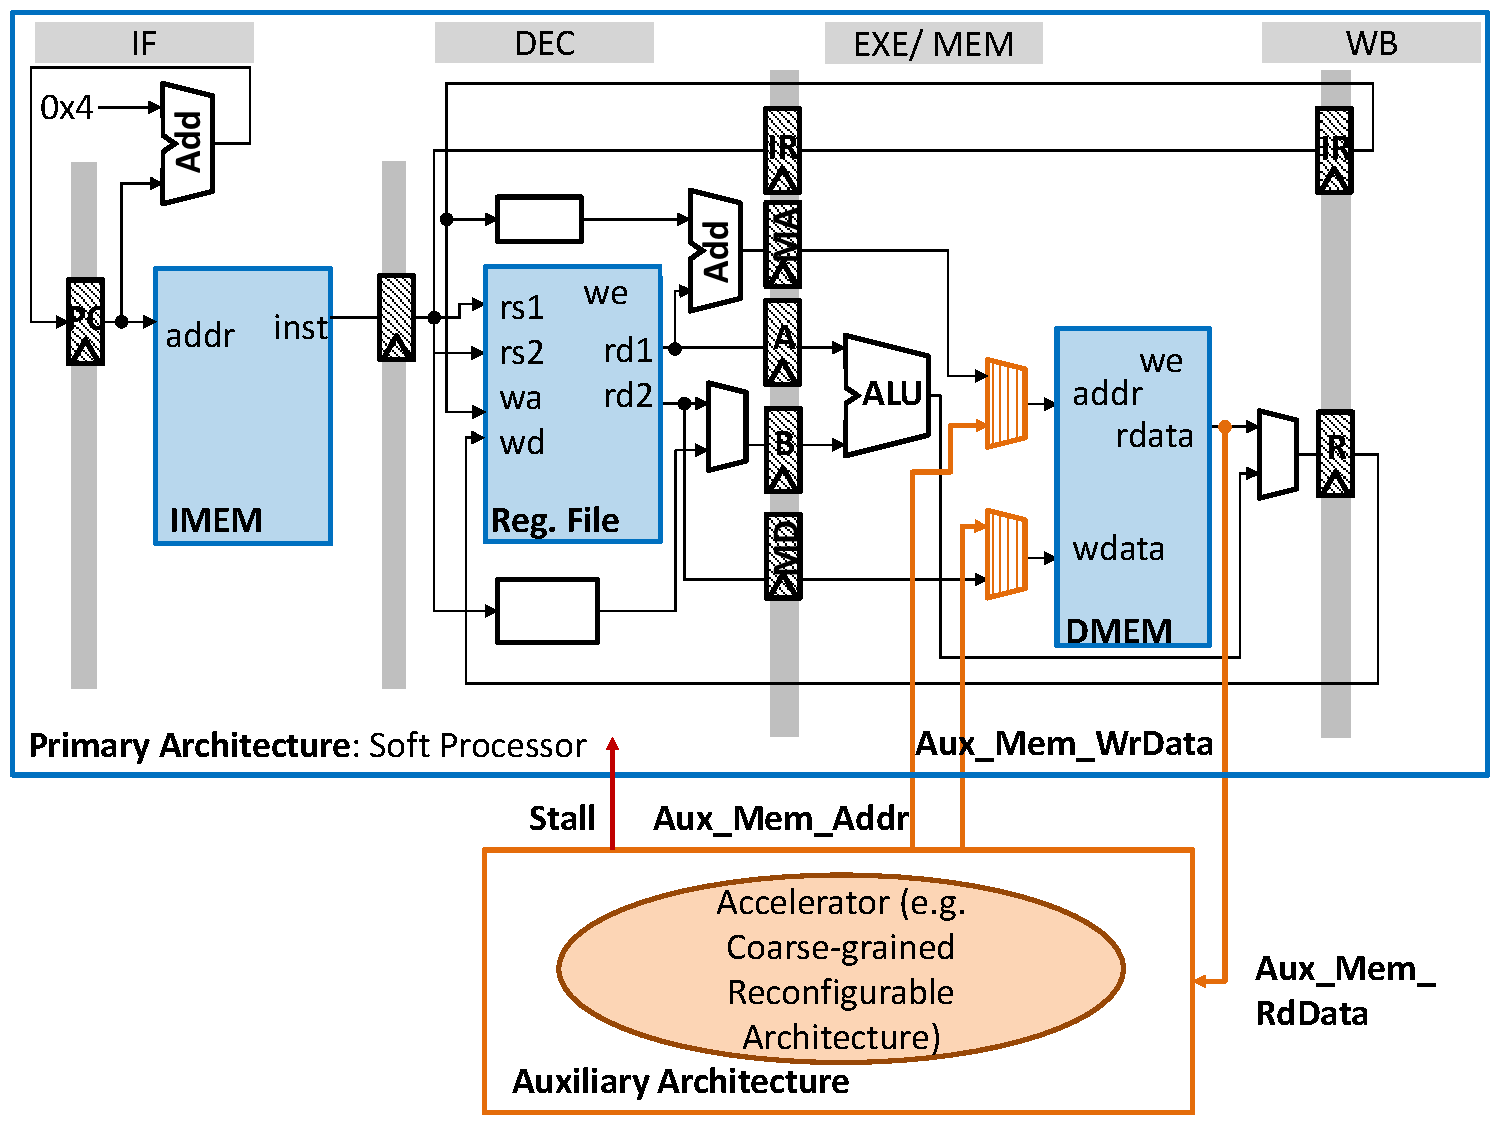
\includegraphics[width=3.3in]{tightly_coupled}
    \caption{High-level diagram of the proposed tightly-coupled architecture.}
    \label{fig:tightly}
\end{figure}

\figref{fig:tightly} displays a high-level diagram of the proposed tightly-coupled architecture. This design consists of two entities where an accelerator can be integrated with the single-issue, in-order processor pipeline by sharing the data memory (DMEM). To ensure correct execution flow, control signal is fed from the accelerator to the processor control path so that the pipeline is stalled correctly when the accelerator is carrying out execution.

\subsection{The Soft Processor}
%As the processor is usually responsible for 10\% time of the entire FPGA overlay execution, it is imperative to have the processor being relatively small in size. 
%As the processor is implemented as part of the FPGA overlay framework, it is imperative to have the processor being relatively small in size. 

In order to reduce substantial resource consumption while maintaining certain efficiency, the soft processor is designed as a 4-stage pipeline by integrating the execution-stage and memory-stage together. This eliminates the load-use hazard where a LOAD instruction is followed by an instruction that uses the value which is just transferred from DMEM to Register File.

In spite of the above advantage, since the memory-stage is now merged with the execution-stage and the memory address needs to be ready before the load/store instruction reaches DMEM, an extra 32-bit adder is placed at the end of the decode-stage. This could incur extra resource consumption and additional pipeline delay.

We found that, from the synthesis results, the proposed 4-stage processor consumes 18\% fewer amounts of FPGA registers and LUTs when compared with the traditional 5-stage pipeline. We believe that this reduction is important for portability and compatibility concerns, especially when the soft processor is ported onto the legacy FPGA devices which could be intrinsically small in size. Also, the additional delay incurred by the extra adder could be partly compensated  by the two additional multiplexers which are placed in front of DMEM.

Moreover, as the benefit of using a virtual layer of overlay architecture on FPGA rests on improving designer's productivity while providing certain customization capabilities, the proposed soft processor can also be customized in terms of the IMEM and DMEM size. Developers can change the memory sizes by modifying a few lines of macro or execute a program that comes along with the soft processor design package.

It is important to note that, in order to further minimize FPGA resource consumptions, components that are not strictly necessary for processor overlay execution are removed from the current implementation. These components include the Control Status Registers (CSR) and their corresponding logic. Future versions of the processor implementation will incorporate the CSR back and will provide tools to allow developers to remove them during the processor customization.

\begin{table}
\begin{center}
\caption{The format of \code{BAA} instruction.}
\label{tab:baa}
%\vspace{5pt}
\renewcommand{\arraystretch}{0.75}% Tighter
\begin{tabular}{|c|c|c|c|c|}
\multicolumn{1}{c}{\code{31\hspace{9mm}20}}%2.3mm as 1 space
 & \multicolumn{1}{c}{\code{19\hspace{4mm}15}}
 & \multicolumn{1}{c}{\code{14\hspace{2mm}12}}
 & \multicolumn{1}{c}{\code{11\hspace{4mm}7}}
 & \multicolumn{1}{c}{\code{6\hspace{7mm}0}}\\
\hline
\code{imm[11:0]}&\code{rs1}&\code{funct3}&\code{-}&\code{opcode}\\
\hline

\multicolumn{1}{c}{\code{12}}
 & \multicolumn{1}{c}{\code{5}}
 & \multicolumn{1}{c}{\code{3}}
 & \multicolumn{1}{c}{\code{5}}
 & \multicolumn{1}{c}{\code{7}}\\

\multicolumn{1}{c}{\code{offset[11:0]}}
 & \multicolumn{1}{c}{\code{base}}
 & \multicolumn{1}{c}{\code{width}}
 & \multicolumn{1}{c}{\code{-}}
 & \multicolumn{1}{c}{\code{BAA}}\\
\end{tabular}
\end{center}
\end{table}

\begin{table}
\begin{center}
\caption{The format of \code{RPA} instruction.}
\label{tab:rpa}
%\vspace{5pt}
\renewcommand{\arraystretch}{0.75}% Tighter
\begin{tabular}{|c|c|c|c|c|}
\multicolumn{1}{c}{\code{31\hspace{9mm}20}}%2.3mm as 1 space
 & \multicolumn{1}{c}{\code{19\hspace{4mm}15}}
 & \multicolumn{1}{c}{\code{14\hspace{2mm}12}}
 & \multicolumn{1}{c}{\code{11\hspace{4mm}7}}
 & \multicolumn{1}{c}{\code{6\hspace{7mm}0}}\\
\hline
\code{imm[11:0]}&\code{rs1}&\code{funct3}&\code{-}&\code{opcode}\\
\hline

\multicolumn{1}{c}{\code{12}}
 & \multicolumn{1}{c}{\code{5}}
 & \multicolumn{1}{c}{\code{3}}
 & \multicolumn{1}{c}{\code{5}}
 & \multicolumn{1}{c}{\code{7}}\\

\multicolumn{1}{c}{\code{offset[11:0]}}
 & \multicolumn{1}{c}{\code{base}}
 & \multicolumn{1}{c}{\code{width}}
 & \multicolumn{1}{c}{\code{-}}
 & \multicolumn{1}{c}{\code{RPA}}\\
\end{tabular}
\end{center}
\end{table}

\subsection{The Tightly-coupled Architecture}
In order to support direct memory access and allow zero-overhead transfers of control, the soft processor is tightly-coupled with the hardware accelerator as illustrated in \figref{fig:tightly}.
In the proposed framework, Multiple Runtime Architecture Computer(MURAC) model~\cite{murac} is adopted to handle the transfer of control when the execution is switched from one architecture to another.

%In order to have the soft-processor tightly-coupled with the CGRA, we need to investigate how the execution can be switched from one architecture to another. In other words, the mechanisms involved during the transfer of control in runtime execution must be well-defined. This is to provide a unified programming model for designers and facilitate compilation and execution on the mixed-architecture in FPGA overlay.

%\subsubsection{MURAC}
%In the proposed framework, Multiple Runtime Architecture Computer (MURAC)~\cite{murac} is employed to implement the above mechanism. MURAC is a unified machine model that considers heterogeneous computing architecture system as a single idealized processor with morphable instruction execution units. That is, the idealized processor can morph its architecture anytime during the runtime for the sake of the performance benefits. It provides an abstraction to programmers by utilizing different computational architectures during runtime to a level similar to the ISA for a specific processor, which abstracts away the low-level details of the hardware structures.


The execution model of the tightly-coupled architecture follows naturally from the MURAC model where the proposed 4-stage pipeline is defined as the \emph{primary architecture} while the hardware accelerator is defined as the \emph{auxiliary architectures}. Switching between these two architectures in runtime is achieved by the Branch-Auxiliary Architecture (\code{BAA}) and Return-To-Primary-Architecture (\code{RPA}) machine instructions. Logically, a MURAC machine contains only one address space that is shared between two architectures.



\subsubsection{Custom Instruction-set Extension}
To apply MURAC machine for the proposed tightly-coupled architecture, custom instruction-set is used to implement the \code{BAA} and \code{RPA} instructions.

Custom instruction-set extension~\cite{riscv_spec} is an important feature in RISC-V \code{RV32I} in the sense that it provides opportunity for designers to integrate other hardware modules such as accelerators onto a standard RISC-V processor. It also provides a unified programming model along various and future RISC-V processor designs, which makes it easier to leverage software development efforts for the ISA toolchain during the processor customization process.


\subsubsection{\code{BAA} and \code{PRA} Instructions Format}
In the proposed architecture, opcode space \emph{custom-0} is selected to implement the \code{BAA} and \code{RPA} instructions. The format of this opcode is defined to be \code{inst[6:0]==0001011}. For the benefits of regularity and simplicity of the decoding hardware, both instructions follow the format of I-type instruction.

\tabref{tab:baa} displays the the format of \code{BAA} instruction which resembles the format as in \code{LOAD} instruction. The fields \code{base} and \code{offset} are added together to form a memory address location. It represents an address location that points to an array of data. This address is passed to the auxiliary architecture, i.e. accelerator during the execution of the \code{BBA} instruction.

The array passed to the auxiliary architecture acts like the command line arguments in any \code{C/C++} program. It stores up the data that is needed by accelerator. The first data represents the number of elements inside the array.


The field \code{width}, on the other hand, is used to distinguish between the \code{BAA} and \code{RPA} instructions, as they share similar encoding. The format of the \code{RPA} instruction is shown in \tabref{tab:rpa}.

The fields \code{base} and \code{offset} in \code{RPA} instruction are added together to form a return memory address. This instruction acts like a return instruction where the program is unconditionally jumped to \code{\code{base+offset}}. Currently, the processor will branch to the address \code{(PC+4)} after the auxiliary architecture finishes its execution. %However, in some scenarios, the processor can adopt the broad definition of an instruction to represent any entity that configures  the machine so as to carry out proper computation. In this case, an FPGA configuration bitfile may be treated as an ultra-long instruction~\cite{quickdough, dehon}, which would make the return address to be \code{PC+length(bitfile)}. 





\subsubsection{Modifications of the Soft Processor}
In the control-path, extra control registers are defined to decode the \code{BAA} and \code{RPA} instructions. These registers are used to recognize the custom instruction with the help of comparators. In addition, stall signals are fed from the auxiliary architecture to the control-path so that the processor would not be executing once the control is passed to accelerator.

On the other hand, when the execution is branched to the auxiliary architecture, the processor pipeline is stalled and components on the data-path such as \code{DMEM} would not be accessed. This makes resource sharing between two architectures possible. In the proposed architecture, \code{DMEM} is designed to be shared with the accelerator. A number of multiplexers are added before the inputs of the \code{DMEM} and the output of \code{DMEM} is also fed to the auxiliary architecture. The control path would assert the correct \code{sel} signal for the multiplexers when the control is branched to auxiliary architecture.
